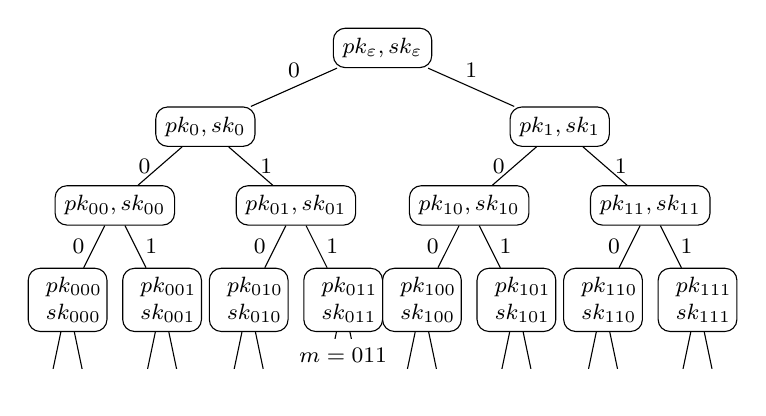
\begin{tikzpicture}[nn/.style={draw,minimum width=1cm, minimum height=0.5cm, rounded corners=1ex},nl/.style={draw,minimum width=0.5cm, minimum height=0.5cm, rounded corners=1ex,circle},level distance=1cm,
level 1/.style={sibling distance=4.5cm}, level 2/.style={sibling distance=2.3cm}, level 3/.style={sibling distance=1.2cm,level distance=1.2cm}, level 4/.style={ sibling distance=0.42cm,level distance=1cm},font=\footnotesize]
%\draw[help lines] (-5,-5) grid (5,1);
\node at (0,0) [nn] {$pk_{\varepsilon},sk_\varepsilon$}
child foreach \x in {0,1} {
  node (n\x) [nn] {$pk_{\x},sk_{\x}$} 
  child foreach \y in {0,1} {
    node (n\x\y) [nn] {$pk_{\x\y},sk_{\x\y}$}
    child foreach \z in {0,1} {
      node (n\x\y\z) [nn,text width=0.55cm] {$pk_{\x\y\z}$ $sk_{\x\y\z}$}
        child foreach \i in {0,1} {
          node (i) {}  
        }
      \ifnum \z = 0
      edge from parent node[midway,left] {$\z$}
      \else
      edge from parent node[midway,right] {$\z$}
      \fi
    }
    \ifnum \y = 0
    edge from parent node[midway,left] {$\y$}
    \else
    edge from parent node[midway,right] {$\y$}
    \fi
  }
  \ifnum \x = 0
  edge from parent node[midway,left,above] {$\x$}
  \else
  edge from parent node[midway,right,above] {$\x$}
  \fi
};
\node (f3) [below of=n011,fill=white,node distance=0.7cm] {$m=011$};
%\draw[-] (f3) -- (n011);
\end{tikzpicture}